\section{Introduction}

\subsection{Motivation}


\begin{frame}{The Rise of online CoPs}
  \begin{itemize}
    \item World Wide Web is a place to meet and exchange information easily
    \item Researches transformed Communities of Practice into online Communities of Practice (CoPs)
          \begin{itemize}
            \item World-wide collaboration
            \item Fast, effortless, information exchange
            \item Community Information Systems (CIS) help structure their work
          \end{itemize}
          %researchers in particular from all over the world can collaborate more easily 
          %what Cops are will be discussed in more detail later.
    \item A CoP is only sustainable, if members continuously provide innovation efforts \cite{RKJa15}
    \item Therefore members need to be aware of their successes and failures to 
    \begin{itemize}
        \item Predict future challenges and opportunities
        \item Ensure the survival of the CoP
    \end{itemize}
  \end{itemize}

\end{frame}

\begin{frame}{Measuring Success}
  \begin{itemize}
    \item Success of CoP relies on success factors
    \item It is difficult to measure and evaluate those factors
          \begin{itemize}
            \item Factors are changing over time \cite{Renz16}
            \item Domain-specific success factors
            \item Less resources in long-tail communities
            \item Time consuming
          \end{itemize}
    \item Traditional success modeling systems automate success evaluation
          \begin{itemize}
            \item Complicated interfaces
            \item Not optimized for collaboration
            \item Do not take mobile context into consideration \cite{Renz16}
          \end{itemize}
  \end{itemize}
\end{frame}

\begin{frame}{Chat platforms}
  %this is why some continuous success modeling systems have been developed
  %however, the problem is that
  Social Networks and chat platforms are used for information exchange
  \begin{itemize}
    \item Intuitive to use
    \item Familiar to most users
    \item Real-time collaboration
    \item Optimized for hand-held devices
  \end{itemize}
  %This shows how chat platforms could address the aforementioned issues
\end{frame}


\subsection{Thesis Goals}

\begin{frame}{Thesis Goals}
  \begin{itemize}
    \item Design a chatbot for success modeling and visualizations for a CIS
    \begin{itemize}
        \item Simplify the success modeling and visualization process 
        % in order to include non-experienced users in the evaluation process
    \end{itemize}
        %   \begin{itemize}
        %     \item Bot should communicate with MobSOS (CCA) %framework
        %     \item Should be deployed with the Social Bot Framework
        %   \end{itemize}
    \item Find out how the bot affects collaboration and success awareness of the community %in contrast to traditional web frontends
  \end{itemize}
\end{frame}







\section{State of the Art}

\subsection{Social Bots}
% \begin{frame}{Social Bots and Chatbots}
%   \begin{block}{Definition}
%     ``A social bot is a computer algorithm that automatically produces content and interacts with humans on social media, \dots'' \cite{FVD*16b}
%   \end{block}
% \end{frame}

\begin{frame}{Social Bots and Chatbots}
  \begin{block}{Definition}
    ``A social bot is a computer algorithm that automatically produces content and interacts with humans on social media, \dots'' \cite{FVD*16b}
  \end{block}
  \ \\
  \begin{itemize}
    % \item integrate automation into daily lives of users  %e.g. Alexa Smart Home, Shopping lists Reminders
    % \item Users interact with bots by voice or chat %in the case of chat: Chatbots
    \item Provide better user experience, compared to traditional interfaces
    \item Engage users in human-like conversations and are therefore more intuitive to use 
    % \item Use Natural Language Understanding to determine users' intent
\end{itemize}
\end{frame}


\subsection{Success in Communities of Practice}
% \begin{frame}{Communities of Practice}
%   \begin{block}{Definition}
%     ``Communities of practice are groups of people who share a concern or a passion for something they do and learn how to do it better as they interact regularly.'' \cite{Weng98}
%   \end{block}
% \end{frame}

\begin{frame}{Communities of Practice}
  \begin{block}{Definition}
    ``Communities of practice are groups of people who share a concern or a
    passion for something they do and learn how to do it better as they interact regularly.'' \cite{Weng98}
  \end{block}
  \ \\
  \begin{itemize}
    % \item CoPs are diverse communities, which study a certain domain
    \item Learner is actively participating in the work of the community
    \begin{itemize}
        \item Naturally gains knowledge in the domain
    \end{itemize}
    \item CoPs make the learning process easier and faster \cite{CuZe05}
    % \item Informal structures with permeable boundaries \cite{RKJa15}
          %informal structures: This means that there are no strict rules about the hierarchy inside a community and they do not follow the same structure as traditional organizations
          %Permeable boundaries: This means that it is not clearly defined which members belong to the CoP and which don't
    % \item CoPs contain sub-communities which can be overlapping
    
          % members can belong to more than one community
  \end{itemize}

   CoPs use Community Information Systems (CIS) to structure their work
\end{frame}


% \begin{frame}{Members of a Communitiy of Practice}
%   \begin{itemize}
%     \item Have various roles
%           \begin{itemize}
%             \item Researchers
%             \item Professionals
%             \item Students
%             \item Hobbyists
%           \end{itemize} %DBIS and ACIS as an example????
%     \item Have different degrees of
%           \begin{itemize}
%             \item Knowledge %Researchers > students
%             \item Interest %Professionals > Hobbyists
%             \item Contribution
%                   \begin{itemize}
%                     \item Core Members %do most of the contribution 
%                     \item Lurkers %only consume but almost no contribution
%                           %study on open Source found that for random projects 22percent contribute. For the top 500 projects: ~90percent don't contribute -> 1% (90-9-1) rule
%                   \end{itemize}
%           \end{itemize}
%     \item Do not have to belong to the same organization
%     \item Share their work through social interaction e.g. online Social Networks %in this case we also talk about an online CoP
%   \end{itemize}
% \end{frame}


\begin{frame}{Success of a CoP}
  \begin{columns}
    \begin{column}[]{0.3\textwidth}
      \begin{itemize}
        \item Communities of Practice need to be aware of their success
              \begin{itemize}
                \item Improve their work
                \item Adjust to current trends
              \end{itemize}
              %Success seems to be a very abstract metric so in order to measure it we build a success model
              \item Success of a Community Information System \textbf{CIS} is formalized through a \emph{Success Model}
              \item Success model is \textbf{distinct} for each community
              %based on the goals that they want to achieve
              %e.g. a community of web developers: front end developers have different goals than backend developers (beautiful animations vs informative (plain html))
      \end{itemize}
    \end{column}
    \begin{column}[]{0.7\textwidth}
      \begin{figure}
        \centering
        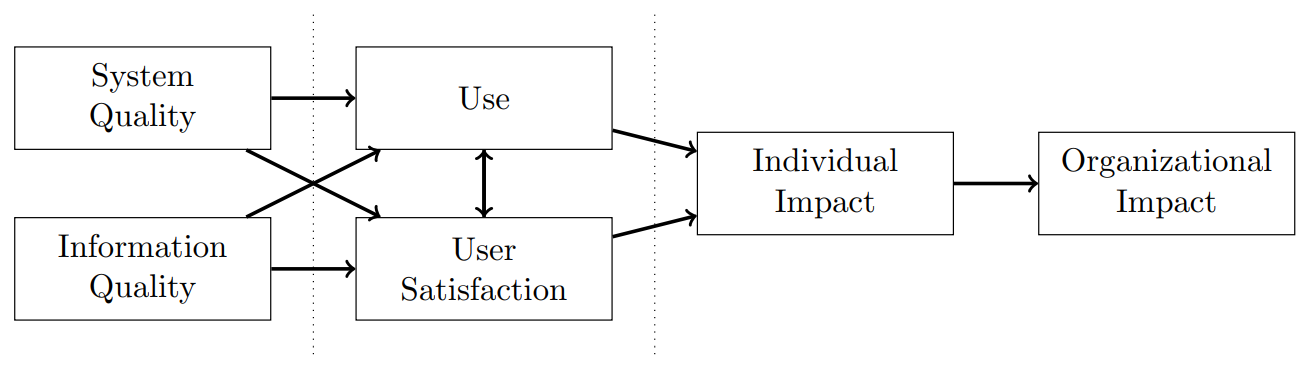
\includegraphics[width=\textwidth]{related_work/deloneMclean.png}
        \caption{CIS Success Model by DeLone and McLean \cite{DeMc92}}
        %13!!!!
      \end{figure}
    \end{column}
  \end{columns}
\end{frame}



\begin{frame}{MobSOS}

  \begin{itemize}
    % \item MobSOS success model is based on the success model of DeLone and McLean
    % \item Core Component of las2peer
    \item Monitors las2peer services \cite{Renz16}
    \begin{itemize}
        \item MobSOS Data Processing
        \item MobSOS Success Modeling
    \end{itemize}
    \item MobSOS Continuous Community Analytics \cite{Kers20} 
    % extends MobSOS
          \begin{itemize}
            \item REST API
            \item GraphQL API
            \item Provides visualizations of MobSOS data
            \item Ability to dynamically add databases
          \end{itemize}
  \end{itemize}
  %The MobSOS cca also allows the addition of Mediabases, which can be used to gather data produced outside the las2peer environment
\end{frame}

% \begin{frame}{Mediabase}
%   \begin{columns}

%     \begin{column}[]{0.4\textwidth}
%       \begin{itemize}
%         \item Proposed to handle Web 2.0 data in a more effective way
%         \item Mediabase includes
%               \begin{itemize}
%                 \item Backend database (DB2 or MySQL)
%                 \item Crawler scripts
%                 \item Monitoring processes
%                 \item Frontend for user interactions
%               \end{itemize}
%       \end{itemize}
%     \end{column}

%     \begin{column}[]{0.6\textwidth}
%       \begin{figure}[h]
%         \centering
%         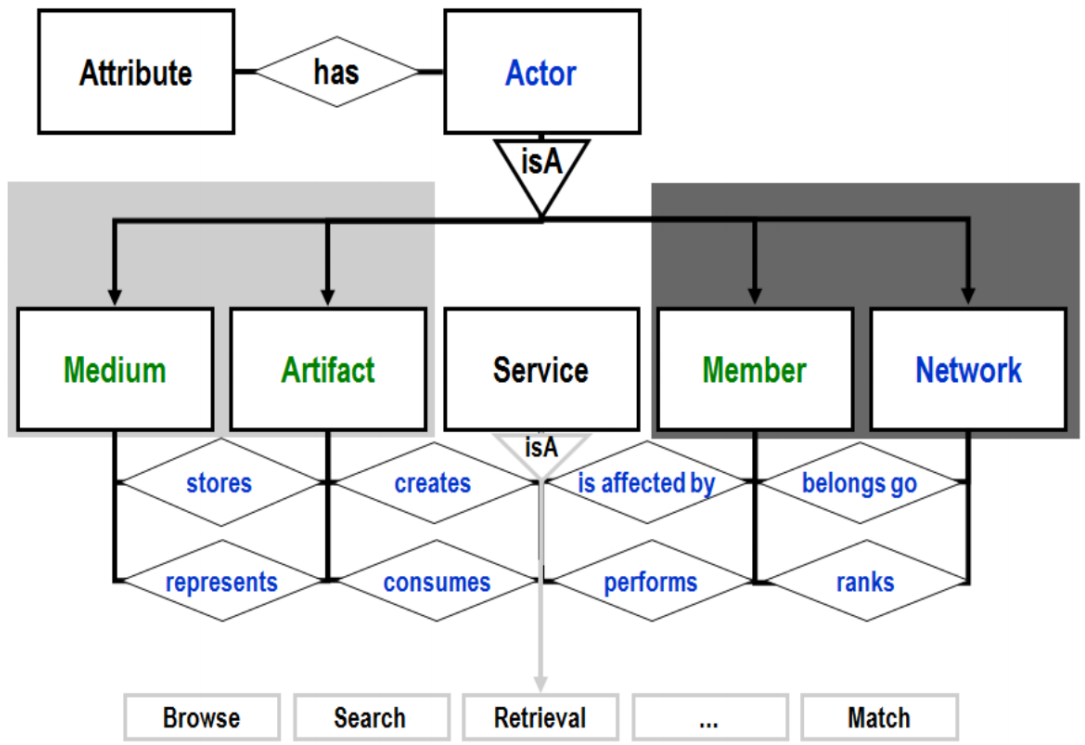
\includegraphics[height=0.8\textheight]{related_work/mediabase.png}
%         \caption{Mediabase Overview \cite{Klam10e}}
%       \end{figure}
%     \end{column}

%   \end{columns}
% \end{frame}



\section{Concept}
\subsection{Use Case}
\begin{frame}{Mensa Communities}
  \begin{itemize}
    \item Community of people frequently visiting the mensa
    \item Community consists of students and university employees
    \item Similar to the concept of Community of Practice %share a concern: food at the canteen. And Interact regularly: Students arguing on which mensa is the best?? Frequent visits to mensa
    % \item Different community levels:
    %       \begin{itemize}
    %         \item Top level: all mensa frequenters in Germany
    %         \item Intermediate level: all mensa frequenters for a University
    %         \item Low level: individual circle of friends, which frequent the canteen together %Members can belong to different circles of friends->overlapping
    %       \end{itemize}
  \end{itemize}
\end{frame}



\begin{frame}{mensabot}
  \begin{columns}
    \begin{column}[]{0.3\textwidth}
      For this community a chatbot called \emph{mensabot} is designed, which can be used to
  \begin{itemize}
    \item Get the menu for a canteen
    \item Rate meals
    \item Query success visualizations designed by the community
    \item Modify the success model of the community
  \end{itemize}
  The chatbot is deployed to Slack
    \end{column}
    \begin{column}[]{0.7\textwidth}
      \begin{figure}
          \centering
          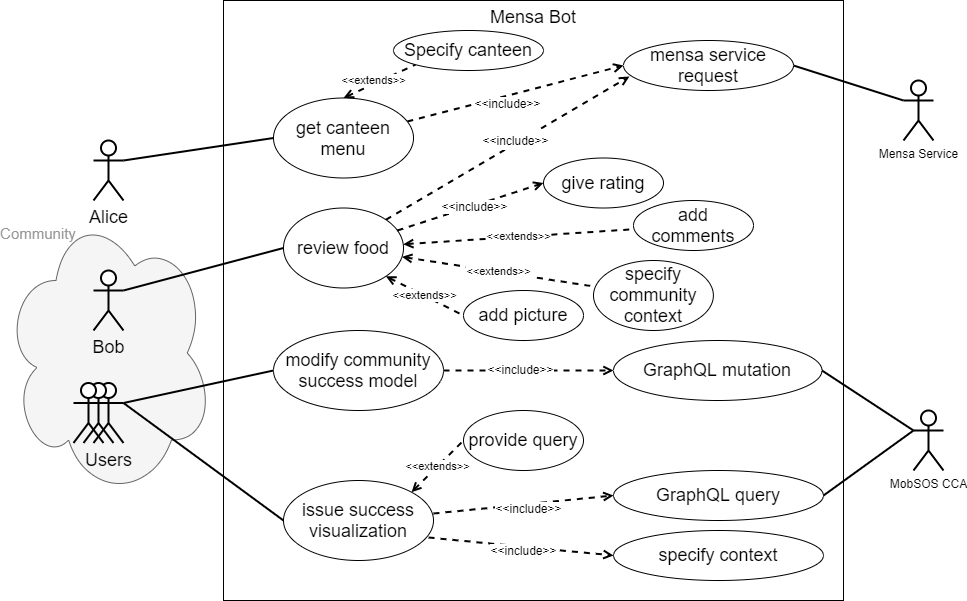
\includegraphics[height=0.85\textheight]{concept/usecase.png}
      \end{figure}
    \end{column}     
  \end{columns}
\end{frame}

% \begin{frame}{Use case diagram for the Chatbot}
%   \begin{figure}
%     \centering
%     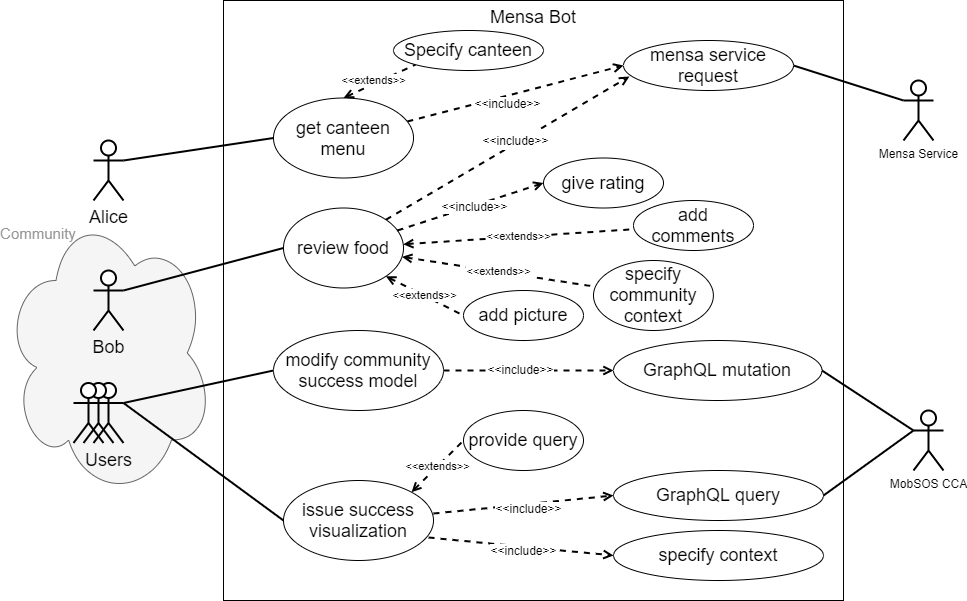
\includegraphics[height=0.85\textheight]{concept/usecase.png}
%   \end{figure}
% \end{frame}

% \subsection{System overview}

% \begin{frame}{System overview}
%   \begin{figure}
%     \centering
%     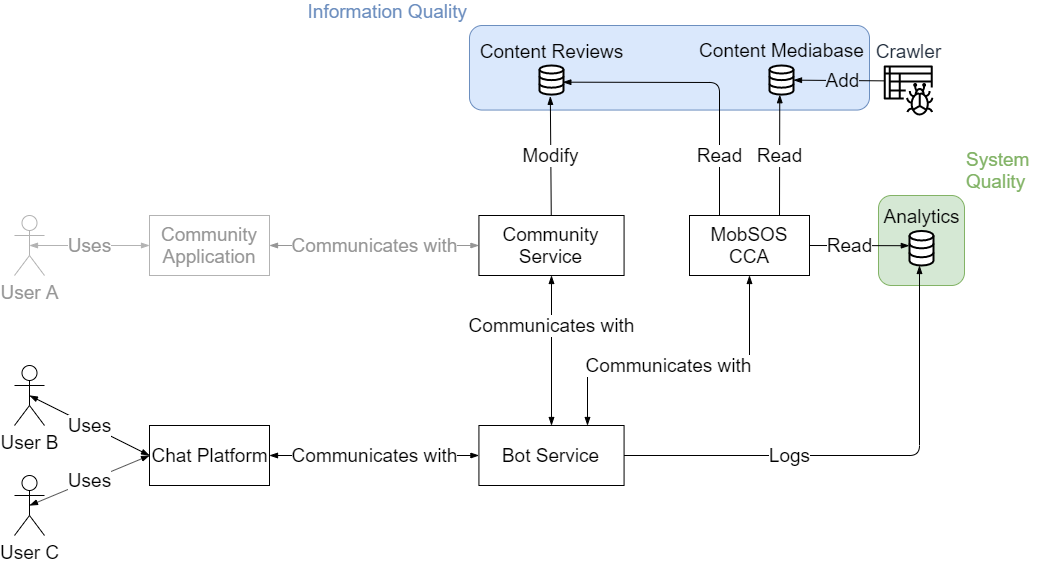
\includegraphics[height=0.85\textheight]{realization/Component_Diagramm.png}

%     \label{fig:sytsemOverview}
%   \end{figure}
% \end{frame}

\section{Realization}

\begin{frame}\begin{columns}
    \begin{column}[]{0.7\textwidth}
      \begin{figure}
        \centering
        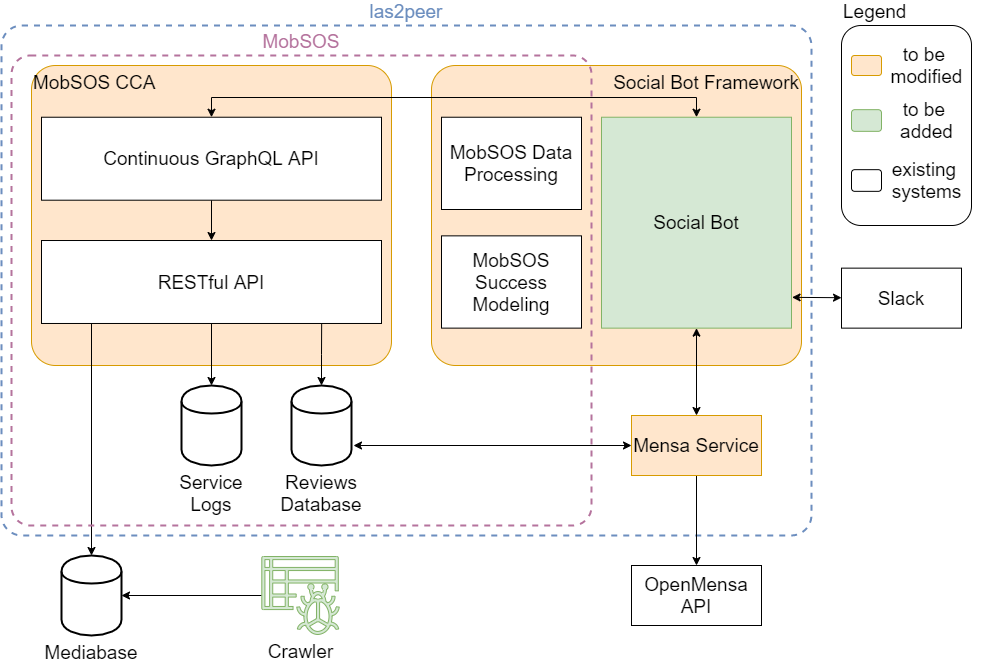
\includegraphics[height=0.9\textheight]{realization/components_overview.png}
        \caption{Overview of the different components}
        \label{fig:componentsOverview}
      \end{figure}
    \end{column}
    \begin{column}[]{0.3\textwidth}
      Technologies:
      \begin{itemize}
        \item Chat Platform (Slack)
        \item las2peer
        \item Social Bot Manager
        \item Mensa Service
        \item MobSOS
              \begin{itemize}
                \item MobSOS CCA GraphQL API
                \item MobSOS CCA REST API
                \item MobSOS Data Processing
                \item MobSOS Success Modeling
              \end{itemize}
        \item Mediabase
              \begin{itemize}
                \item Crawler
              \end{itemize}
      \end{itemize}
    \end{column}
  \end{columns}
\end{frame}

\begin{frame}{Example of a visualization request}
    
    \begin{columns}
        \begin{column}[t]{0.5\textwidth}
            \begin{figure}
                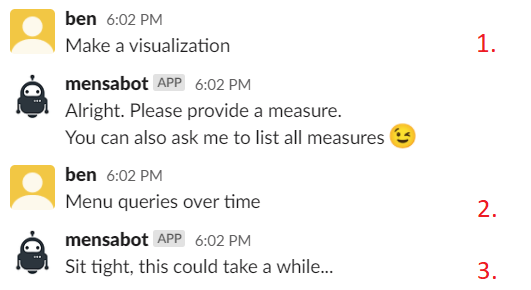
\includegraphics[width=0.9\textwidth]{realization/bot/visual_alt1_anot.png} 
            \end{figure}
        \end{column}
        \begin{column}[t]{0.5\textwidth}
            \begin{enumerate}
              \item Intent visualization is recognized
              \begin{itemize}
                \item Visualization routine is triggered
              \end{itemize}
              \item User message is passed to success modeling service
            \item Success modeling service prepares the visualization
            \begin{itemize}
              \item Extract the measure from the catalog
              \item CCA GraphQL request for data
              \item Data2Chart request to generate chart
            \end{itemize}
            \end{enumerate}
        \end{column}
    \end{columns}
\end{frame}

\begin{frame}{Example of a visualization request}
  \begin{columns}
    \begin{column}[t]{0.5\textwidth}
      \begin{figure}
        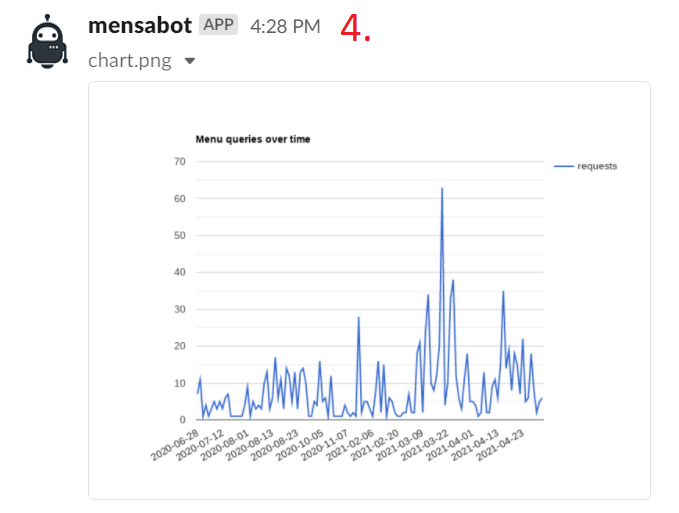
\includegraphics[width=.7\textwidth]{realization/bot/visual_alt2.png} 
      \end{figure}
    \end{column}
    \begin{column}[t]{0.5\textwidth}
      \begin{enumerate}
        \setcounter{enumi}{3}
        \item Resulting chart is sent back to the bot manager
        \\Bot displays the chart in the chat
      \end{enumerate}
    \end{column}
  \end{columns}
\end{frame}

\section{Evaluation}
\begin{frame}{Research Questions}
  \begin{enumerate}
    \item How does the use of chatbots affect the success awareness of the community?
    \item How does it affect collaboration between members?
    % \item Does it improve the user experience in terms of mobility?
  \end{enumerate}
\end{frame}


\begin{frame}{The requirements of the community}
  \begin{itemize}
    \item We conducted a survey to figure out the requirements of the community
    \item Participants were asked to rank success factors based on perceived relevance
    \item Success model contains the most popular success factors
  \end{itemize}
\end{frame}

\begin{frame}{Evaluation tasks}
  \begin{itemize}
    \item Get the menu for a canteen
    \item Make a review
    \item Visualize a success measure from the success model
    \item Get the success model
    \item Update the success model
  \end{itemize}
\end{frame}

\begin{frame}{Evaluation of community service}
  \begin{columns}
    \begin{column}[t]{0.5\textwidth}
      \begin{figure}[H] 
   \centering
    \begin{tikzpicture}
      \begin{axis}
        [xmin=0.9,xmax=5.1,
            label style={font=\footnotesize},
            tick label style={font=\footnotesize},
            yticklabels,
            height=4.5cm,width=8cm,ytick={1,2,3,4,5,6,7},ylabel={Average User Rating }
           ,scatter/classes={
          a={mark=,red!50!black},
          b={mark=,blue!50!black},
          c={mark=,green!50!black},
          d={mark=,white!50!black}
         },title={"I could imagine myself using this bot to get the menu."}]
        
        \addplot[color=blue,
        boxplot prepared={
          median= 4,
          upper quartile=5,
          lower quartile=3,
          upper whisker=5,
          lower whisker=1,
        },
         ] coordinates {}; 
    
         \addplot[scatter,only marks,scatter src=explicit symbolic] 
       table [
         y=y,
         x=x
        ]
    {
    x y 
    4 1 
    
    };
    \node[align=center, text=black]
    at (axis cs:4,1.2) {\scalebox{0.8}{SD=1.5}};
      \end{axis}
    \end{tikzpicture}
   

    \begin{tikzpicture}
        \begin{axis}
            [xmin=0.9,xmax=5.1,
            label style={font=\footnotesize},
            tick label style={font=\footnotesize},
            yticklabels,
            height=4.5cm,width=8cm,ytick={1,2,3,4,5,6,7},ylabel={Average User Rating}
           ,scatter/classes={
          a={mark=,red!50!black},
          b={mark=,blue!50!black},
          c={mark=,green!50!black},
          d={mark=,white!50!black}
         },title={"I could imagine myself using the bot to make reviews."}]
          \addplot[color=blue,
          boxplot prepared={
            median=4,
            upper quartile=5,
            lower quartile=3,
            upper whisker=5,
            lower whisker=1,
          },
           ] coordinates {}; 
      
           \addplot[scatter,only marks,scatter src=explicit symbolic] 
         table [
           y=y,
           x=x
          ]
      {
      x y 
      4 1 
      };
      \node[align=center, text=black]
      at (axis cs:4,1.2) {\scalebox{0.8}{SD=1.27}};
        \end{axis}
      \end{tikzpicture}
      \caption{Usability of the bot to get the menu and write reviews}
      \label{fig:canteenPlot1}
      \end{figure}
    \end{column}
    \begin{column}[t]{0.5\textwidth}
      \begin{itemize}
        \item Participants are aware of the importance of contributions
        \item But: are less inclined to contribute themselves
        % \item This confirms earlier findings which 
        \item Confirms that about 90\% of the community do not contribute \cite{Niel06}
       \item Participants suggested that contributing without receiving anything in return was not attractive to them.
        \item Possible Solution: introduce \emph{Gamification}
        \begin{itemize}
          \item Periodic visualization of Top contributors 
          \item Collect points for making reviews
          \item Special bot functionalities could be unlocked at a certain level e.g.
          \begin{itemize}
            \item Recommendations for canteens
            \item Alerts if a certain dish is served
          \end{itemize} 
        \end{itemize}
      \end{itemize}
    \end{column}
  \end{columns}
\end{frame}

\begin{frame}{Evaluation of success modeling service}
  \begin{columns}
    \begin{column}[t]{0.5\textwidth}
      
\begin{figure}[H] 
    \centering
    \begin{tikzpicture}
      \begin{axis}
        [xmin=0.9,xmax=5.1,
        label style={font=\footnotesize},
        tick label style={font=\footnotesize},
        yticklabels,
        height=4.5cm,width=8cm,ytick={1,2,3,4,5,6,7},ylabel={Average User Rating }
       ,scatter/classes={
      a={mark=,red!50!black},
      b={mark=,blue!50!black},
      c={mark=,green!50!black},
      d={mark=,white!50!black}
     },title={"I could imagine using the bot to add measures to the success model"}]
        \addplot[color=blue,
        boxplot prepared={
          median= 5,
          upper quartile=5,
          lower quartile=4,
          upper whisker=5,
          lower whisker=2,
        },
         ] coordinates {}; 
    
         \addplot[scatter,only marks,scatter src=explicit symbolic] 
       table [
         y=y,
         x=x
        ]
    {
    x y 
    4.5 1 
    
    };
    \node[align=center, text=black]
    at (axis cs:4.5,1.2) {\scalebox{0.8}{SD=1.38}};
      \end{axis}
    \end{tikzpicture}
\caption{}
\label{fig:SuccPlot1}
    
   
    
\end{figure}

    \end{column}
    \begin{column}[t]{0.5\textwidth}
      \begin{itemize}
        \item Visualizations were intuitive to participants
        \item However: Participants wished to get more information about measures
        \item The success model itself seemed not very intuitive to users.
        \begin{itemize}
          \item Provide general information of the meaning of elements in the success model.
        \end{itemize}
        \item Overall, both success modeling and visualizations were well received
      \end{itemize}
    \end{column}
  \end{columns}
\end{frame}

\begin{frame}{Conclusion}
  \begin{itemize}
    \item Chatbot was evaluated using the System Usability Scale (SUS)
    \begin{itemize}
      \item SUS score of 71,7 \textbf{Good}
    \end{itemize}
    \item Overall, the chatbot is useful for simple tasks
    \item Chatbot increases the success awareness in the community
    \item Most community members are aware that contributions help the community.
    \item However, they are less inclined to contribute to the community themselves.
    \item We need to introduce incentives to increase contributions
  \end{itemize}
\end{frame}

\begin{frame}{Conclusion}
  \Huge{\centerline{Thank you for listening! Any questions?}}
\end{frame}


